	\documentclass[aspectratio=43]{beamer}
\usepackage[english]{babel}
\usepackage{amsthm}
\usepackage{amsfonts}
\usepackage{amsmath}
\usepackage{amssymb}
\usepackage{mathtools}
\usepackage{bbm}
\usepackage{pgfplots}
\usepackage{tikz}
%\usepackage{physics}
\usepackage{calligra}
\usepackage{csquotes}
%\usepackage{tensor}
\usepackage[thicklines]{cancel}
\usepackage{tcolorbox}
%\usepackage{pstricks}
\usepackage[backend=biber, bibstyle=nature, sorting=nty, citestyle=numeric-comp]{biblatex} %Custom bibliography
    \addbibresource{bib.bib} %Load references
\usepackage{chronology}
\usepackage{msc}

\DeclareMathAlphabet{\mathcalligra}{T1}{calligra}{m}{n}
\DeclareFontShape{T1}{calligra}{m}{n}{<->s*[2.2]callig15}{}
\newcommand{\scriptr}{\mathcalligra{r}\,}
\newcommand{\boldscriptr}{\pmb{\mathcalligra{r}}\,}
\def\rc{\scriptr}
\def\brc{\boldscriptr}
\def\hrc{\hat\brc}
\newcommand{\ie}{\emph{i.e.}} %id est
\newcommand{\eg}{\emph{e.g.}} %exempli gratia
\newcommand{\rtd}[1]{\ensuremath{\left\lfloor #1 \right\rfloor}}
\newcommand{\dirac}[1]{\ensuremath{\delta \left( #1 \right)}}
\newcommand{\diract}[1]{\ensuremath{\delta^3 \left( #1 \right)}}
\newcommand{\e}{\ensuremath{\epsilon_0}}
\newcommand{\m}{\ensuremath{\mu_0}}
\newcommand{\V}{\ensuremath{\mathcal{V}}}
\newcommand{\prnt}[1]{\ensuremath{\left(#1\right)}} %parentheses
\newcommand{\colch}[1]{\ensuremath{\left[#1\right]}} %square brackets
\newcommand{\chave}[1]{\ensuremath{\left\{#1\right\}}}  %curly brackets
\newcommand\eqdef{\stackrel{\mathclap{\normalfont \tiny\mbox{\textrm{def}}}}{=}}
\useoutertheme{infolines}
\useinnertheme{rectangles}
\usefonttheme{professionalfonts}


\definecolor{blue2}{HTML}{045FB4}
\definecolor{green2}{HTML}{46C235}
\definecolor{red2}{HTML}{EE4848}
\definecolor{violet2}{HTML}{A647E5}
\definecolor{orange2}{HTML}{FF7425}
\definecolor{darkred}{HTML}{5C2020}
\definecolor{gray}{HTML}{303030}
\definecolor{yellow}{HTML}{f0be52}
\definecolor{lightdarkgold}{HTML}{EEBC1D}

\renewcommand{\CancelColor}{\color{darkred}}

\makeatletter
\newcommand{\mybox}[1]{%
  \setbox0=\hbox{#1}%
  \setlength{\@tempdima}{\dimexpr\wd0+13pt}%
  \begin{tcolorbox}[colback=gray,colframe=gray,boxrule=0.5pt,arc=4pt,
      left=6pt,right=6pt,top=6pt,bottom=6pt,boxsep=0pt,width=\@tempdima]
    \textcolor{yellow}{#1}
  \end{tcolorbox}
}
\makeatother


\pgfplotsset{my style/.append style={axis x line=middle, axis y line=
middle, xlabel={$x$}, ylabel={$y$}, axis equal }}


\usecolortheme[named=gray]{structure}
\usecolortheme{sidebartab}
\usecolortheme{orchid}
\usecolortheme{whale}
\setbeamercolor{titlelike}{parent=structure, bg=structure, fg=white}
\setbeamercolor{section in toc}{fg= white}
\setbeamercolor{subsection in toc}{fg= white}
%\setbeamercolor*{sidebar}{fg=red2,bg=gray!15!white}

\setbeamercolor{item projected}{bg=yellow, fg = gray}
\setbeamertemplate{enumerate items}[default]
\setbeamertemplate{navigation symbols}{}
\setbeamercolor{local structure}{fg=yellow}

\setbeamercolor{alerted text}{fg=white}
\setbeamercolor{block title}{bg = yellow}
\setbeamercolor{block title alerted}{bg=red2}
\setbeamercolor{block title example}{bg=green2}
\setbeamercolor{background canvas}{bg=gray}
\setbeamercolor{normal text}{bg=gray,fg=white}


\setbeamertemplate{footline}
        {
      \leavevmode%
      \hbox{%
      \begin{beamercolorbox}[wd=.333333\paperwidth,ht=2.25ex,dp=1ex,center]{author in head/foot}%
        \usebeamerfont{author in head/foot}\insertshortauthor~~(\insertshortinstitute)
      \end{beamercolorbox}%
      \begin{beamercolorbox}[wd=.333333\paperwidth,ht=2.25ex,dp=1ex,center]{title in head/foot}%
        \usebeamerfont{title in head/foot}\insertshorttitle
      \end{beamercolorbox}%
      \begin{beamercolorbox}[wd=.333333\paperwidth,ht=2.25ex,dp=1ex,center]{date in head/foot}%
        \usebeamerfont{date in head/foot}\insertshortdate{}%\hspace*{2em}

    %#turning the next line into a comment, erases the frame numbers
        %\insertframenumber{} / \inserttotalframenumber\hspace*{2ex} 

      \end{beamercolorbox}}%
      \vskip0pt%
    }


\setbeamertemplate{blocks}[rectangle]
\setbeamercovered{dynamic}




%\setbeamercolor{author}{fg=yellow}
%\setbeamercolor{title}{fg = yellow}
%\setbeamerfont{title}{size=\Large, series=\bfseries}
%\setbeamerfont{author}{size=\footnotesize}
%\setbeamerfont{date}{size=\small}


\setbeamertemplate{section page}
{
	\begin{centering}
		\begin{beamercolorbox}[sep=27pt,center]{part title}
			\usebeamerfont{section title}\insertsection\par
			\usebeamerfont{subsection title}\insertsubsection\par
		\end{beamercolorbox}
	\end{centering}
}





%\setbeamertemplate{subsection page}
%{
%	\begin{centering}
%		\begin{beamercolorbox}[sep=12pt,center]{part title}
%			\usebeamerfont{subsection title}\insertsubsection\par
%		\end{beamercolorbox}
%	\end{centering}
%}

\newcommand{\hlight}[1]{\colorbox{violet!50}{#1}}
\newcommand{\hlighta}[1]{\colorbox{darkred!50}{#1}}


    \setbeamertemplate{background} 
    {
        
\includegraphics[width=\paperwidth,height=\paperheight]{images/fond1.jpg}
    }
\title{Privacy Preserving Cryptographic Toolbox } %->->->->-> Check hyperref title <-<-<-<-<-
\subtitle{A survey with applications to Sovereign Identity}
\author[R. Dubois]{\textcolor{yellow}{Renaud Dubois}}
\institute[LIT]{
    \textcolor{white}{Ledger}%
    \\%
    \textcolor{white}{Innovation Team}%
} %You can change the Institution if you are from somewhere else
\date{\today}
%\logo{\includegraphics[width= 0.05\textwidth]{images/logo.png}}

\begin{document}
    
    \frame{\titlepage}
%%%%%%%%%%%%         
    \begin{frame}{Summary}
    
        \tableofcontents
        
%         Reed-Solomon Proximity (RP) Problem: Given oracle access to a Reed-Solomon code $f:S\rightarrow\mathbb{F}$, the Reed-Solomon Proximity Problem asks that a verifier $V$ distinguishes between two cases with high probability: \begin{itemize}
%                                                                                                                                                                                                                                           \item $$f\in \textbf{RS}[\mathbb{F},S,\rho]$$
%                                                                                                                                                                                                                                           \item $f$ is $\delta$-far pairwise Hamming distance from all $$f^\prime\in\textbf{RS}[\mathbb{F},S,\rho], f\neq f^\prime$$.
%                                                                                                                                                                                                                                          \end{itemize} 
   
    \end{frame} 
%%%%%%%%%%%% 
    
%%%%%%%%%%%%%%%%%%%%%%%%%%%%%%%%%%%%%%%%%%%%%%%%
%%%%%%%%%%%%%%%%%%%%%%%%%%%%%%%%%%%%%%%%%%%%%%%%       
    \section{Identity, Privacy  and Sovereignty }
    \frame{\sectionpage}
    \subsection{Identity}
%%%%%%%%%%%%%%%%%%%%%%%%%%%%%%%%%%%%%%%%%%%%%%%%    
    \begin{frame}{Identity}
     
%      \begin{definition}[Wikipedia]
%      Identity is the qualities, beliefs, personality traits, appearance, and/or expressions that characterize a person or group.
%      \end{definition}
     
        \only<1>{ 
          \begin{definition}[Wikipedia]
     Identity is the qualities, beliefs, personality traits, appearance, and/or expressions that characterize a person or group.
     \end{definition}
        }
        \only<2>{
        \begin{definition}[{[CL16]}]
      Digital identity is a collection of attributes someone knows about.
     \end{definition}
     \begin{center}
     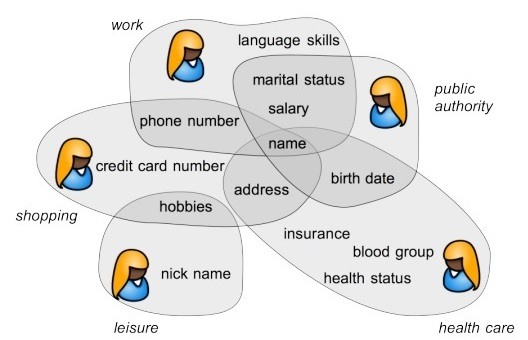
\includegraphics[width=7.5cm]{images/identity.jpg}
     \end{center}
     From now on we will refer Identity, Privacy and Sovereignty as Digital ones.
        }
    
    \end{frame}

%%%%%%%%%%%%%%%%%%%%%%%%%%%%%%%%%%%%%%%%%%%%%%%%

    \subsection{Privacy}
    \begin{frame}{Privacy}
    
    \begin{definition}[Wikipedia]
    Privacy is the ability of an individual or group to seclude {\color{blue2}{themselves}} or {\color{red}{information}} about themselves, and thereby express themselves {\color{red}selectively}.
    \end{definition}
 
    \begin{block}{Vires in Numeris}
    \only<1>
    {
     \begin{tabular}{ll}
        \begin{minipage}{4cm}
         ~\\~\\~\\~\\
        \end{minipage}
        &
        \begin{minipage}{5.5cm}
         ~\\~\\~\\~\\
        \end{minipage}
      \end{tabular}  
    }
    \only<2-3>
    {
    \begin{tabular}{ll}
        \begin{minipage}{4cm}
          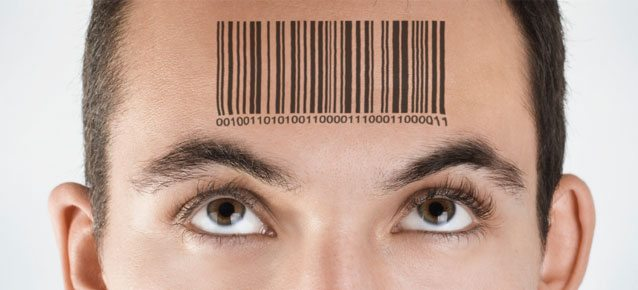
\includegraphics[width=4cm]{images/privacy.jpeg}
        \end{minipage}
        &
        \begin{minipage}{5.5cm}
         \begin{itemize}
          \item Alphabet+Meta : 3G€
          \item Nym's Fund : 0.3 G€
          \item RGPD : 1G€ in France
         \end{itemize}

        \end{minipage}
    \end{tabular}  
    }
    \end{block}
    
    
     \only<1-2>
    {
    \begin{exampleblock}{Definition (IND-PRIV2)}
     \begin{tabular}{ll}
        \begin{minipage}{4cm}
         ~\\~\\~\\~\\
        \end{minipage}
        &
        \begin{minipage}{5.5cm}
        ~\\~\\~\\~\\
        \end{minipage}
      \end{tabular}  
      \end{exampleblock}
    }
    \only<3>
    {
    \begin{alertblock}{Definition (IND-PRIV2)}
     
   
    \begin{tabular}{ll}
        \begin{minipage}{4cm}
          \includegraphics<3>[width=4cm]{images/blackhole.jpg}
        \end{minipage}
        &
        \begin{minipage}{5.5cm}
         \begin{itemize}
          \item Privacy domain is unclear : no RGS or unique primitive
          \item Survey (Kahoot)
         \end{itemize}
        \end{minipage}
    \end{tabular}  
    
    \end{alertblock}

     }
    
    \end{frame}
    %Selon une étude de la CDC, 21 % des internautes fournissent volontairement des données erronées
      %404 : Not Found
%%%%%%%%%%%%   
  \begin{frame}{Privacy at Ledger}
  
  \begin{block}{Use cases}
    \begin{itemize}
     \item Ledger Database : update of Ledger Live links accounts
     \item Device ID : links desktops and phones
     \item Ledger Live :  genuine check
     \item Registering to a conference with Ether Fee
    \end{itemize}
    \end{block}
   
   \begin{alertblock}{Noob Remarks}
    \begin{itemize}
     \item We have privacy legal, but no privacy tech's or dungeon
     
    \end{itemize}   
   \end{alertblock}

   Take offline solutions as priority, reduce collected information at maximum.

  \end{frame}

%%%%%%%%%%%%   



%%%%%%%%%%%%   

  \subsection{Self Sovereignty}
  \begin{frame}{Self Sovereign Identity (SSI)}
  
  \begin{definition}[Wikipedia]
  Self-sovereign identity (SSI) is an approach to {\bf digital identity} that gives individuals {\color{red} control} of their digital identities.
  \end{definition}
  
  \begin{center}
  
\includegraphics[width=6cm]{images/takeback.jpg}
  \end{center}

     
  In the litterature, the Cryptographic solution is referred as Anonymous Credentials (AC) or Attribute Based Signature. The notion of control implies that the user decides which attribute is revealed.

  \end{frame}

    
    %%%%%%%%%%%   
    \subsection{Anonymous Credentials}
  \begin{frame}{Anonymous Credentials}
  
  \begin{center}
  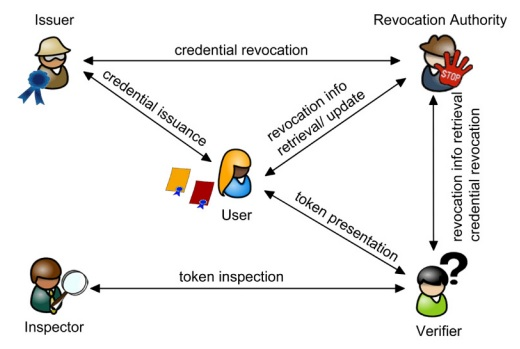
\includegraphics[width=8cm]{images/anonymouscredentials.jpg}
  \end{center}

  \end{frame}

 \begin{frame}{Anonymous Credentials Recipee}
 
 \begin{center}
 \textcolor{yellow}{\fbox{Ingredients}} 
 \end{center}

 \fbox{\parbox{\textwidth}{

 \begin{itemize} 
  \item Commitment : Digital sealed envelope, polynomial Commitment, Functional Commitment. Enables range-proof (Monero), serial number hiding (Zerocoin), universal proofs.
  \item Signatures with efficient protocols : Proof friendly, Structure Preserving, Group, Linkable \ldots
  \item Zero Knowledge Proof : proof a Knowledge of a value, without revealing it. From single value to universal.
 \end{itemize}
 }}
 
 \end{frame}
 
%%%%%%%%%%%%   

    \section{Privacy-Preserving Cryptographic Toolbox}
     \frame{\sectionpage}

     \subsection{Commitments}
     
%%%%%%%%%%%%%%%%%%%%%%%%%%%%%%%%%%%%%%%%%%%%%     
 \begin{frame}{Basic Commitment}
 
  \only<1>{
   Digital Analog of Sealed envelope.
  \begin{center}
  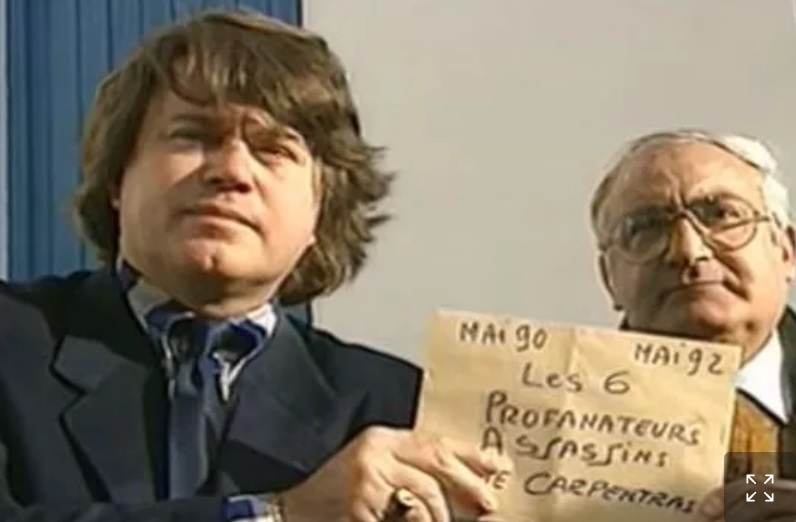
\includegraphics[width=8cm]{images/commitment.jpg}
  
  \tikzset{>=latex}
  \end{center}
  }
  \only<2>
  {
  
  $
    \begin{array}{c c c}
&&\\
         
\begin{minipage}{4cm}
\begin{center}
 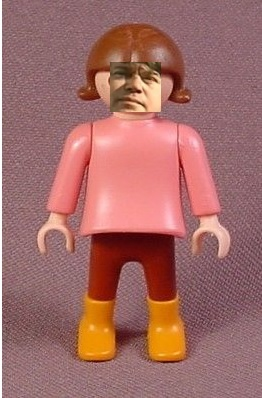
\includegraphics[width=1cm]{images/alice.jpg}
 \end{center}
\end{minipage}
&&
     
\begin{minipage}{4cm}
\begin{center}
 
\includegraphics[width=1cm]{images/bob.jpg}
 \end{center}
\end{minipage}
\\
\text{\textsf{Prover}} & & \text{\textsf{Verifier}} \\
com = H(m,r) &  \xrightarrow{\hspace{1em}
\begin{minipage}{1cm}
\begin{center}
 
\includegraphics[width=1cm]{images/closed.jpg}
 \vspace{0.05cm} $com$
 \end{center} 
\end{minipage}  \hspace{1em}} & \\

 & \xrightarrow{\hspace{1em}
\begin{minipage}{1cm}
\begin{center}
 
\includegraphics[width=1cm]{images/opened.jpg}
 \vspace{0.05cm} $Open(m,r)$
 \end{center} 
\end{minipage}  \hspace{1em}} &  com \stackrel{?}{=}H(m,r)

\end{array}$
  }

\end{frame}
%%%%%%%%%%%%%%%%%%%%%%%%%%%%%%%%%%%%%%%%%%%%%     

    

%%%%%%%%%%%%%%%%%%%%%%%%%%%%%%%%%%%%%%%%%%%%%     
 \begin{frame}{Pedersen Additive Homomorphic Commitment}
 totocs
 \end{frame}
 

\section{Pictures}
\begin{frame}
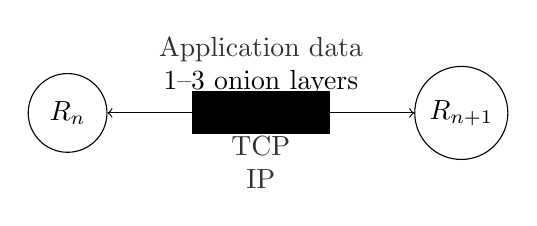
\begin{tikzpicture}

\node[circle,draw,minimum size=1cm] (R1) at (0, 0) {$R_n$};
\node[circle,draw,minimum size=1cm] (R2) at (5, 0) {$R_{n+1}$};

\draw[<->] (R1.east) -- node [midway, fill=black] (line) {\phantom{TLS layer}} (R2.west);

\node[align=center] at (line) {{\color{gray} Application data}\\1--3 onion
                    layers\\TLS layer\\{\color{gray}TCP}\\{\color{gray} IP}};

\end{tikzpicture}

\end{frame}
\begin{frame}



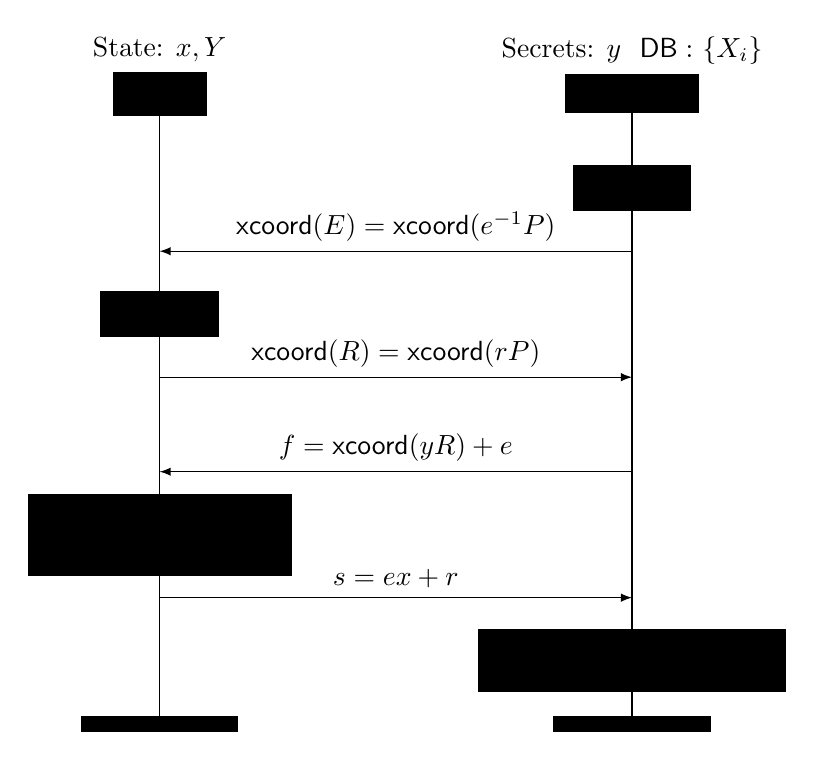
\begin{tikzpicture}[box/.style={draw,fill=black,align=center}]
\draw [line width=2mm] (0,0) -- ++(2,0) coordinate[midway](L1)
(6,0) -- ++(2,0) coordinate[midway](R1);
\draw (L1) -- ++ (0,8) 
node[box,pos=0.3] (L1a) {$e=f-\texttt{xcoord}(rY)$\\ $Ee\stackrel{?}{=}P$}
node[box,pos=0.65] (L1b) {$r\in_RZ_\ell^*$}
node[box,pos=1,label=above:{State: $x,Y$}] (L1c) {Tag $T$}
coordinate[pos=0.2] (X1) coordinate[pos=0.55] (X2);
\draw (R1) -- ++ (0,8) 
node[box,pos=0.1] (R1a) {$X=e^{-1}(sP-R)\stackrel{?}{\in}\mathsf{DB}$}
node[box,pos=0.85] (R1b) {$e\in_RZ_\ell^*$}
node[box,pos=1,label=above:{Secrets: $y$~~$\mathsf{DB}:$ $\{X_i\}$}] (R1c) {Reader $T$}
coordinate[pos=0.4] (X3) coordinate[pos=0.75] (X4);
\draw[-latex] (X1) -- (X1 -| R1) node[midway,above]{$s=ex+r$};
\draw[-latex] (X2) -- (X2 -| R1) node[midway,above]{$\mathsf{xcoord}(R)=\mathsf{xcoord}(rP)$};
\draw[-latex] (X3) -- (X3 -| L1) node[midway,above]{$f=\mathsf{xcoord}(yR)+e$};
\draw[-latex] (X4) -- (X4 -| L1) node[midway,above]{$\mathsf{xcoord}(E)=\mathsf{xcoord}(e^{-1}P)$};
\end{tikzpicture} 
 \end{frame}

 
%     \section{Blocks and Colors}
 \frame{\sectionpage}

\begin{frame}{Color}

\begin{itemize}
    \item \textcolor{blue2}{That's the blue2 color}
    \item \textcolor{green2}{That's the green2 color}
    \item \textcolor{red2}{That's the red2 color}
    \item \textcolor{violet2}{That's the violet2 color}
    \item \textcolor{orange2}{That's the orange2 color}
    \item \textcolor{yellow}{That's the yellow color}
\end{itemize}
    
\end{frame}

\begin{frame}{Blocks}
\begin{block}{begin block}
There's a block
\end{block}

\begin{alertblock}{begin alertblock}
    there's a alert block 
\end{alertblock}

\begin{exampleblock}{begin example block}
here comes example
\end{exampleblock} 

\end{frame}


\begin{frame}{Blocks}
    
\begin{theorem}
    Here comes a theorem
\end{theorem}

\begin{proof}
    Here comes the proof
\end{proof}


    
\end{frame}

%      
     \section{boxes and columns}
 \frame{\sectionpage}
 
\begin{frame}{Box}
    \begin{center}
        \textcolor{yellow}{\fbox{phrase inside box}} 

    \bigskip    
    
    \fbox{\parbox{\textwidth}{A big box\\ \[ 
    \{R^n_{\alpha}(0) \; | \; n \in \mathbb{N}\} = \{n\alpha \; \mathrm{mod}\;1 \; | \; n \in \mathbb{N}\} \]
    é denso em \([0,1)\). }}
 \end{center}
\end{frame}
    
\begin{frame}{Two Columns entire page}
\small

\begin{columns}
\begin{column}{0.5\textwidth}
\tiny \pause \textcolor{yellow}{Obs:} \(\alpha \eqdef \log b \in \mathbb{R}\backslash\mathbb{Q}\)
\small \pause 
   \begin{align*}
    R_\alpha \colon [0,1) &\longrightarrow [0,1) \\
                      x   &\longmapsto x + \alpha \; \mathrm{mod}\;1           
\end{align*}
\pause 
\small 
Here we can write some text Here we can write some text Here we can write some text Here we can write some text Here we can write some text  Here we can write some text  Here we can write some text
\end{column}
\begin{column}{0.5\textwidth}  %%<--- here
\pause 
\[R^n_\alpha(x) \eqdef R_\alpha \overbrace{\circ \ldots \circ }^{n} R_\alpha(x)\]

\pause 

Here we can write some text Here we can write some text Here we can write some text Here we can write some text Here we can write some text  Here we can write some text  Here we can write some text

\bigskip 

\footnotesize 
\textcolor{yellow}{\fbox{\parbox{\textwidth}{Question??????????? tell me if you want}}} 
\bigskip

the answer is 
\pause 
\textcolor{green2}{YES!!!!} \textcolor{green2}{because that that and that} or..

\bigskip 

The answer is \textcolor{red2}{NO!!!!} \textcolor{red2}{because that that and that}

\end{column}
\end{columns}

\end{frame}
    
    
\begin{frame}{Table and minipage}

\begin{center}
\begin{tabular}{|l|l|l|l|l|l|l|l|l|l|l|l|l|}
\hline
\(n\) & 1  & 2 & 3 & 4 & 5 & 6 & 7 & 8 & 9 & 10 & 11 & \ldots       \\ \hline
\(2^n\) & \textcolor{yellow}{2} & \textcolor{yellow}{4} & \textcolor{yellow}{8} & \textcolor{yellow}{1}6 & \textcolor{yellow}{3}2 & \textcolor{yellow}{6}4 & \textcolor{yellow}{1}28 &  \textcolor{yellow}{2}56 & \textcolor{yellow}{5}12 & \textcolor{yellow}{1}024 & \textcolor{yellow}{2}048 & \ldots    \\ \hline
\end{tabular}
\end{center}

\pause 

\bigskip

\begin{center}
\textcolor{yellow}{\fbox{o dígito 1 é mais frequente que o dígito 3?}}
\bigskip

\pause \tiny Spoiler: \textcolor{green2}{YES}.

\end{center}


\pause 
\bigskip
\small 
\
\pause 
\begin{minipage}{0.47\textwidth}
    Um conjunto de números satisfaz a \emph{\textcolor{yellow}{lei de Benford}} se o primeiro dígito \(d \in \{1,2,3,4,5,6,7,8,9\} \) ocorre com a seguinte proporção 
\end{minipage}
\begin{minipage}{0.47\textwidth}
    \centering  \textcolor{yellow}{\(P(d) = \log\bigg(1+ \frac{1}{d}\bigg) \)} 
\end{minipage}
\end{frame}


    
    %\section{Equations and Figure}
     
    \frame{\sectionpage}
    
    \begin{frame}{Ordinary Differential Equations}
        \uncover<+->{\begin{equation*}
            \dv{x} y(x) + \frac{1}{CR} y(x) = 0
        \end{equation*}}
        
        \uncover<+->{\begin{equation}
            \dv[2]{x} y(x) + \gamma \dv{x} y(x) + \omega_0^2 y(x) = f(x)
        \end{equation}}
    \end{frame}
    
    \begin{frame}{}
        \uncover<+>{\begin{equation*}
            \dv[2]{x} y(x) + \gamma \dv{x} y(x) + \omega_0^2 y(x) = f(x)
        \end{equation*}}
        \uncover<+>{\[ \Downarrow \]
        \begin{equation*}
            \colch{\dv[2]{x} + \gamma \dv{x} + \omega_0^2} y(x) = f(x)
        \end{equation*}}
        \uncover<+>{\[ \Downarrow \]
        \begin{equation*}
            y(x) = \frac{f(x)}{\dv[2]{x} + \gamma \dv{x} + \omega_0^2}
        \end{equation*}}
    \end{frame}
    
    \begin{frame}{Imagem}
        \centering
        \includegraphics[width = 0.8\textwidth]{images/coke.jpg}\\
        \footnotesize \textcolor{yellow}{Figure:} Some words about the figure here
    \end{frame}
    
 
    \begin{frame}{See how is cool the fourier serie}
        \uncover<+>{\begin{equation*}
            \mathcal{F}[f](\xi) = \hat{f}(\xi) = \frac{1}{\sqrt{2\pi}} \int_{-\infty}^{+\infty} f(x) e^{-i x \xi} \dd{x}
        \end{equation*}}
        \uncover<+>{\begin{equation*}
            \mathcal{F}^{-1}[\hat{f}](x) = f(x) = \frac{1}{\sqrt{2\pi}} \int_{-\infty}^{+\infty} \hat{f}(\xi) e^{i x \xi} \dd{\xi}
        \end{equation*}}
    \end{frame}
    
    \begin{frame}{Quality Control}
        \uncover<+>{\begin{equation*}
            \widehat{(f + \alpha g)}(\xi) = \frac{1}{\sqrt{2\pi}} \int_{-\infty}^{+\infty} \prnt{f(x) + \alpha g(x)} e^{-i x \xi} \dd{x}
        \end{equation*}}
        \uncover<+>{\[ \Downarrow \]
        \begin{equation*}
            \widehat{(f + \alpha g)}(\xi) = \frac{1}{\sqrt{2\pi}} \int_{-\infty}^{+\infty} f(x) e^{-i x \xi} \dd{x} + \frac{\alpha}{\sqrt{2\pi}} \int_{-\infty}^{+\infty} g(x) e^{-i x \xi} \dd{x}
        \end{equation*}}
        \uncover<+>{\[ \Downarrow \]
        \begin{equation*}
            \widehat{(f + \alpha g)}(\xi) = \hat{f}(\xi) + \alpha \hat{g}(\xi)
        \end{equation*}}
    \end{frame}
    
    \begin{frame}{Quality Control}
        \uncover<+>{\begin{equation*}
            \widehat{f'}(\xi) = \frac{1}{\sqrt{2\pi}} \int_{-\infty}^{+\infty} f'(x) e^{-i x \xi} \dd{x}
        \end{equation*}}
        \uncover<+>{\[ \Downarrow \]
        \begin{equation*}
            \widehat{f'}(\xi) = \eval{\frac{f(x) e^{-ix\xi}}{\sqrt{2\pi}}}^{+\infty}_{-\infty} + i\xi \cdot \frac{1}{\sqrt{2\pi}} \int_{-\infty}^{+\infty} f(x) e^{-i x \xi} \dd{x}
        \end{equation*}}
        \uncover<+>{\[ \Downarrow \]
        \begin{equation*}
            \widehat{f'}(\xi) = i\xi \widehat{f}(\xi)
        \end{equation*}}
    \end{frame}
    
    \begin{frame}{Quality Control}
        \centering
        \textcolor{green2}{\huge{The inverse does work}}
        
        \normalsize{for appropriate functions} 
        
        \tiny{and, sometimes, the Fourier Transform of a function is not in the same set as the original function, but let's forget about this since we do not know a decent theory of integration}
    \end{frame}
 
    
    %\section{graphs and other tikz}
 \frame{\sectionpage}
 
\begin{frame}{Drawning within tikz}
    \tikzset{every picture/.style={line width=0.75pt}} %set default line width to 0.75pt        

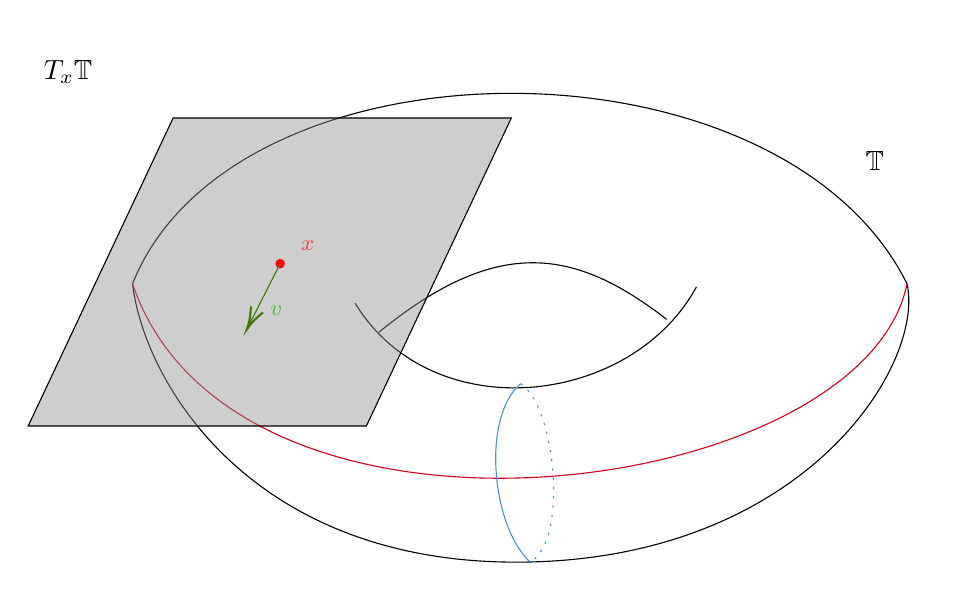
\begin{tikzpicture}[x=0.75pt,y=0.75pt,yscale=-1,xscale=1]
%uncomment if require: \path (0,486); %set diagram left start at 0, and has height of 486

%Curve Lines [id:da9595099437611456] 
\draw    (233.23,183.24) .. controls (252.87,215.34) and (288.86,227.45) .. (323.09,223.22) .. controls (353.65,219.45) and (382.81,202.65) .. (397.65,175.44) ;
%Curve Lines [id:da6932103982097759] 
\draw    (244.67,197.26) .. controls (301.86,150.51) and (339.03,156.74) .. (383.35,191.03) ;
%Curve Lines [id:da7053828945347995] 
\draw    (126,173.88) .. controls (131.72,222.2) and (184.62,311.04) .. (317.59,307.92) .. controls (450.55,304.8) and (507.74,212.85) .. (499.16,173.88) ;
%Curve Lines [id:da583602680611125] 
\draw    (126,173.88) .. controls (174.61,52.32) and (437.68,50.76) .. (499.16,173.88) ;
%Curve Lines [id:da5190289437371578] 
\draw [color={rgb, 255:red, 208; green, 2; blue, 27 }  ,draw opacity=1 ]   (126,173.88) .. controls (175,318) and (478,278) .. (499.16,173.88) ;
%Curve Lines [id:da5494113181101443] 
\draw [color={rgb, 255:red, 74; green, 144; blue, 226 }  ,draw opacity=1 ]   (313,222) .. controls (294,238) and (299,291) .. (317.59,307.92) ;
%Curve Lines [id:da8828117501564781] 
\draw [color={rgb, 255:red, 74; green, 144; blue, 226 }  ,draw opacity=1 ] [dash pattern={on 0.84pt off 2.51pt}]  (313,222) .. controls (330,233) and (336,298) .. (317.59,307.92) ;
%Shape: Parallelogram [id:dp02778297397005436] 
\draw  [fill={rgb, 255:red, 144; green, 144; blue, 144 }  ,fill opacity=0.44 ] (145.57,94) -- (308.5,94) -- (238.68,242.38) -- (75.75,242.38) -- cycle ;
%Shape: Circle [id:dp8371213746664339] 
\draw  [color={rgb, 255:red, 253; green, 1; blue, 1 }  ,draw opacity=1 ][fill={rgb, 255:red, 255; green, 0; blue, 0 }  ,fill opacity=1 ] (195.13,164.19) .. controls (195.13,163.08) and (196.02,162.19) .. (197.13,162.19) .. controls (198.23,162.19) and (199.13,163.08) .. (199.13,164.19) .. controls (199.13,165.29) and (198.23,166.19) .. (197.13,166.19) .. controls (196.02,166.19) and (195.13,165.29) .. (195.13,164.19) -- cycle ;
%Straight Lines [id:da21346648436809335] 
\draw [color={rgb, 255:red, 65; green, 117; blue, 5 }  ,draw opacity=1 ]   (197.13,164.19) -- (181.9,194.22) ;
\draw [shift={(181,196)}, rotate = 296.88] [color={rgb, 255:red, 65; green, 117; blue, 5 }  ,draw opacity=1 ][line width=0.75]    (10.93,-3.29) .. controls (6.95,-1.4) and (3.31,-0.3) .. (0,0) .. controls (3.31,0.3) and (6.95,1.4) .. (10.93,3.29)   ;

% Text Node
\draw (501,122.4) node [anchor=north west][inner sep=0.75pt]    {$\ $};
% Text Node
\draw (478,109) node [anchor=north west][inner sep=0.75pt]   [align=left] {\(\mathbb{T}\)};
% Text Node
\draw (82,65) node [anchor=north west][inner sep=0.75pt]   [align=left] {\(T_x\mathbb{T}\)};
% Text Node
\draw (206,152) node [anchor=north west][inner sep=0.75pt]   [align=left] {\textcolor{red2}{{\footnotesize \(x\)}}};
% Text Node
\draw (191.06,183.09) node [anchor=north west][inner sep=0.75pt]   [align=left] {{\footnotesize \textcolor{green2}{\(v\)}}};

\end{tikzpicture}

    
\end{frame}



\begin{frame}{It's possible plotting graphs with pgfplots and tikz}

\centering
\begin{tikzpicture}
\begin{axis}
\addplot[color=yellow]{exp(x)};
\end{axis}
\end{tikzpicture}
%Here ends the 2D plot

%Here ends the 3D plot

\end{frame}

\begin{frame}{Plotting 3d}
%Here begins the 3D plot
\centering
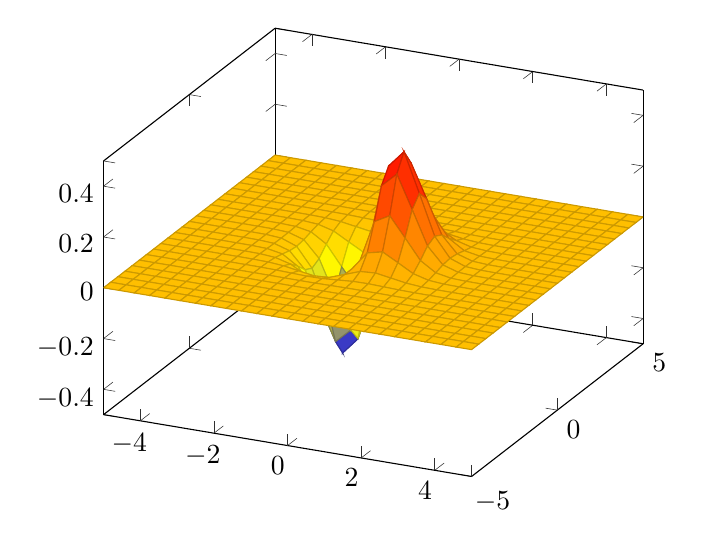
\begin{tikzpicture}
\begin{axis}
\addplot3[
    surf,
]
{exp(-x^2-y^2)*x};
\end{axis}
\end{tikzpicture}
\end{frame}

    
    
 %   \section*{References} %You can remove this if you do not want to use it
 %       \nocite{Djairo} \nocite{PhilPanof} \nocite{Fleming} \nocite{Shankar}
 %       \begin{frame}{References}
 %           \printbibliography
 %       \end{frame}

    \section{}
    \begin{frame}{}
        \centering
            \Huge\bfseries
        \textcolor{yellow}{Questions ?}
            
\includegraphics[width=12cm]{images/questions.jpg}
     
    \end{frame}
\end{document}

% https://en.wikipedia.org/wiki/Privacy
% [CL16]: Concepts Around Privacy-Preserving Attribute-Based CredentialsJan Camenisch  https://hal.archives-ouvertes.fr/hal-01276046/document
